\section{Experimental Results}
\label{text:experiments/results}

\subsection{Experimental Setup}
- walking speed \cite{Bohannon1997}


\subsection{Interactive Objective Function Performance}
Next to the interactive objective function $J_{int}(\cdot)$, which is described in Section \ref{text:approach/objective/interactive}, there are several other ways to formulate it. Instead of taking the full trajectory distribution into account for computing the a distance measure between the unconditioned $\distwo[]$ and the conditioned trajectory distribution $\dist[]$, it can be approximated by computing the expected value over sample pairs. Consequently, the distance measure breaks down to a weighted sum over $L_2$-norms for each discrete time-step within the time horizon and for every trajectory pair, which are efficient to compute.

\begin{equation}
D_{int}^{sp} = \sum_{samples} \sum_T ||\xpedwo[s]_t - \xped[s]_t||_2
\end{equation}

The samples are deterministic trajectories, and can be numerically differentiated efficiently, using central difference expressions. As previously described, it might be more meaningful to compare velocity or acceleration instead of positions.

\begin{align}
J_{int, sa}^{k} &= \sum_{samples} \sum_T ||\ddxpedwo[s]_t - \ddxped[s]_t||_2	 \\
J_{int, sv}^{k} &= \sum_{samples} \sum_T ||\dxpedwo[s]_t - \dxped[s]_t||_2	 \\
J_{int, sp}^{k} &= \sum_{samples} \sum_T ||\xpedwo[s]_t - \xped[s]_t||_2
\label{eq:interaction_diff}	
\end{align}

Although quite intuitive, it turns out that a sample-wise objective is hard to optimize. This has two predominant reasons: Firstly, it intrinsically relies on a trade-off between computational feasibility (to compute many times per second for an online optimization) and capability to capture the properties of the underlying real distributions sufficiently well. Secondly, when randomly drawn samples are used, stochasticity is introduced into the objective function, which might lead to a different objective value even when evaluated with the same input. When the distribution's means are used instead, the distribution's uncertainty is disregarded.
\newline
In the following, the projection-probability-based interactive loss function in Equation \ref{eq:objective_interact_prob} is compared against the alternative difference-based objectives, presented above in \ref{eq:interaction_diff}. Due to the previously explained limitations instead of sampled trajectories, merely the mean trajectory is being used, thereby neglecting the prediction's variance. For the comparison, a Monte Carlo simulation is used for a set of customly defined scenarios. Due to the uncertainty evolved in the environment dynamics, the performance is evaluated over 10 test runs each. To exclude interactive effects occurring due to other parts of the optimization, other than the compared objective functions, the safety constraint is not used in this experiment. \\ 

\begin{table}[!ht]
\begin{center}
\begin{tabular}{c|c|c|c|c|c|c}
\bf Interactive Objective & \bf MPE & \bf RTD & \bf RCE & \bf ETT & \bf TGD & \bf MSD \\
\hline
diff\_pos & 0.33 & 0.99 & 0.32 & 0.0 & 0.24 & 0.94 \\
\hline
diff\_vel & 0.29 & 0.98 & 0.51 & 0.0 & 0.26 & 1.16 \\
\hline
diff\_acc & 0.21 & 0.98 & 0.55 & 0.0 & 0.27 & 1.24 \\ 
\hline
\rowcolor{baseline_color}
without & 0.31 & 1.0 & 0.27 & 0.0 & 0.23 & 1.08 \\ 
\hline
\rowcolor{our_color}
projection & 0.01 & 0.92 & 0.79 & 0.8 & 0.39 & 1.44 
\end{tabular}
\end{center}
\label{table:interactive_objective}
\end{table}

The experiments show the effect of the interactive objective function: It trades off the required travel time to reach the goal position with increasing the safety and "ease" of the interaction by reducing the pedestrian's efforts as well as increasing the minimal separation distance. Figure \ref{img:interactive_comp} displays the solution trajectories for an exemplary scenario. While the projection-probability objective accomplishes to just increase distance when necessary, but gets on track afterwards, the alternative formulations either fail to establish a sufficient distance to the pedestrian (comp. the second or third image, associated with diff\_pos and diff\_vel) or cannot recover afterwards as in case for the acceleration difference objective.

\begin{figure}[!ht]
\begin{center}
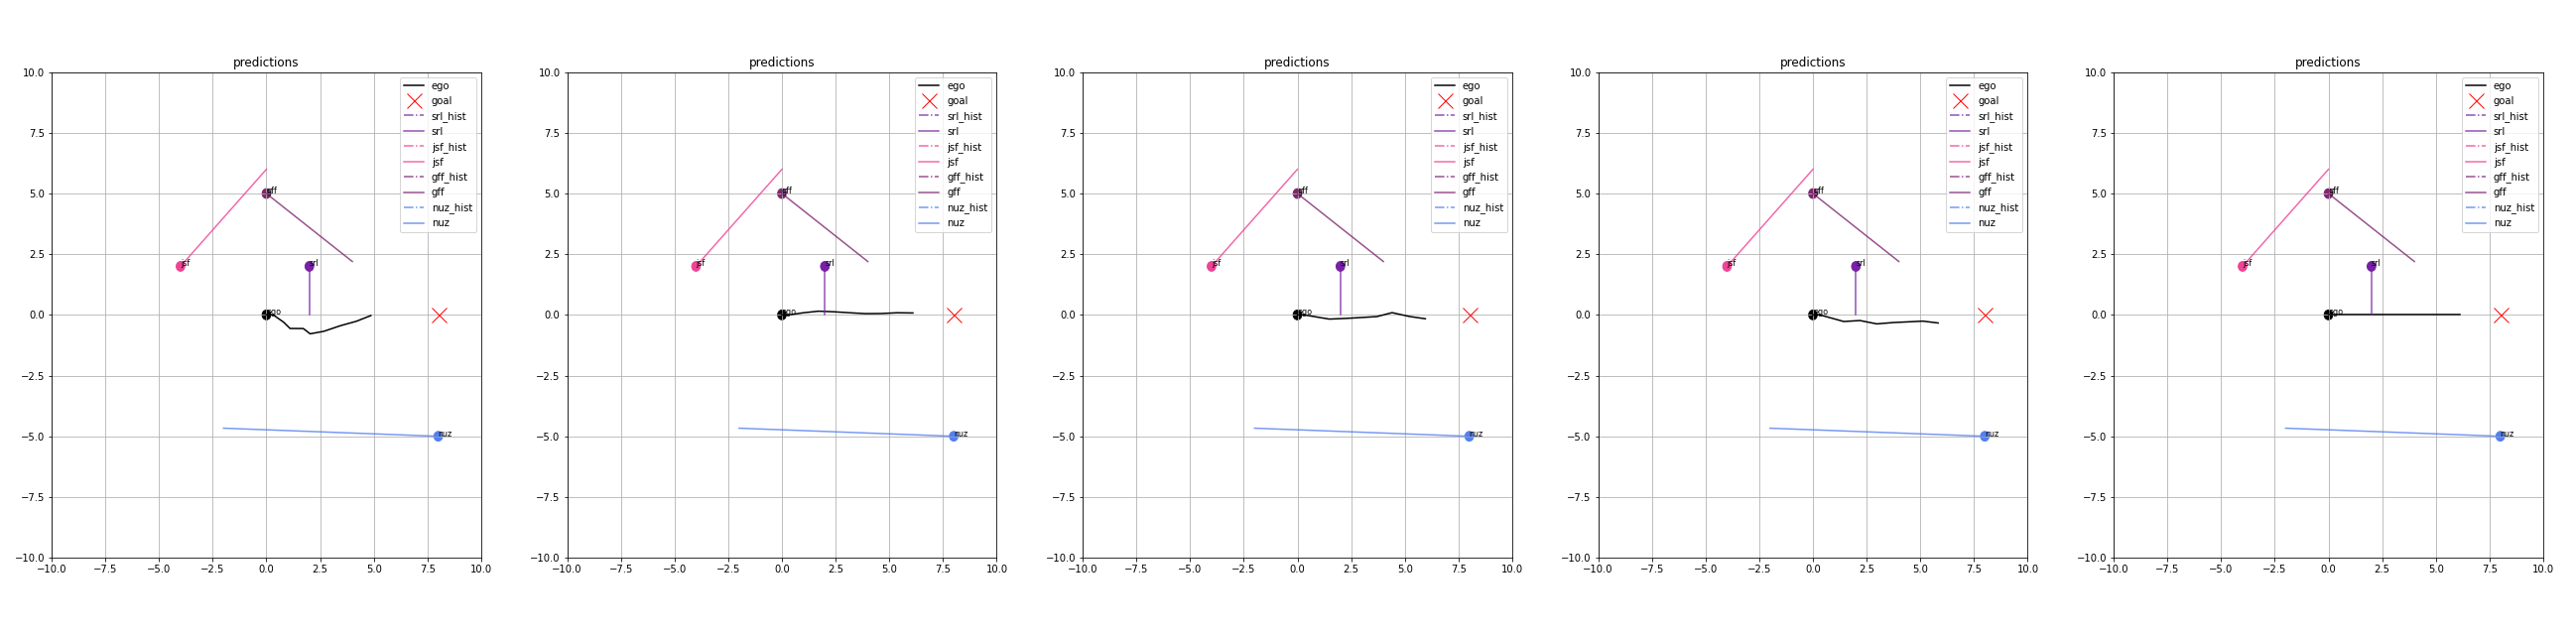
\includegraphics[width=\textwidth]{images/inter_comp_multi.png}
\captionof{figure}{Example solution trajectories for different interactive objective function, beginning from the left: projection, diff\_pos, diff\_vel, diff\_acc, without interactive loss function}
\label{img:interactive_comp}
\end{center}
\end{figure}

